\chapter{Metodología}

\section{Revisión bibliográfica}

\subsection{Objetivos de la revisión}
La revisión bibliográfica en este trabajo tiene como propósito comprender el estado actual de los Modelos de Lenguaje a Gran Escala (LLM) e identificar las mejores prácticas en cuanto a la interacción mediante \textit{prompting} en programación informática y composición musical.

\subsection{Fuentes y búsqueda}
Para llevar a cabo esta revisión, se consultarám diversas bases de datos, revistas especializadas y conferencias de relevancia en el ámbito principalmente de la inteligencia artificial y el \textit{prompting}. La publicación de artículos científicos en el área de la inteligencia artificial, y, en concreto, de LLM, es diaria, y debido a que la mayoría de estos trabajos han sido publicados durante 2022 y 2023, no cuentan con revisión por pares u otros mecanismos de verificación de las tesis en ellos contenidas. Por esta razón, sus resultados deben ser tomados con cautela y como líneas abiertas de investigación.

\subsection{Selección y evaluación}
Los criterios utilizados para seleccionar los trabajos incluidos en esta revisión se centraron en la relevancia y actualidad. Se dieron prioridad a trabajos publicados en los últimos meses y aquellos que se centran específicamente en aspectos cruciales de los LLM y la interacción mediante \textit{prompting} y la programación. 

\subsection{Resultados de la revisión}
Los hallazgos más relevantes de esta revisión son discutidos en detalle en el capítulo correspondiente al \hyperref[chap:estado_cuestion]{Estado de la cuestión}. No obstante, es importante destacar que existen múltiples enfoques y técnicas para interactuar con los LLM, y que su aplicación en la composición musical aún se encuentra en una fase exploratoria, al no ser un objetivo primordial de los investigadores en el campo de la generación de código. Por otra parte, la mayoría de los trabajos publicados en el área de la música y los modelos generativos se centran en la generación de música como producto final, con una clara proyección comercial, y no en la interacción con los LLM como herramienta de composición. 

\section{Enfoque, alcance y diseño}

\subsection{Enfoque}

El enfoque de esta investigación es cualitativo, y se centra en la interacción con los LLM como herramienta de composición musical. Se busca comprender y descubrir los procesos creativos que sustentan la interacción con los LLM en la composición musical algorítmica. Aunque nos apoyamos en estudios previos de carácter cuantitativo, especialmente enfocados al campo de la programacion informática, el enfoque de esta investigación busca explorar los modos de interacción entre el compositor y los LLM, y no tanto medir la eficacia de los mismos en la generación de código. 

\subsection{Alcance}
La investigación tiene un \textbf{alcance exploratorio y descriptivo}. Es exploratoria en la medida en que busca comprender y descubrir la aplicación de los LLM en el contexto de la composición musical algorítmica, un campo que aún no ha sido ampliamente estudiado. Al mismo tiempo, se adopta un enfoque descriptivo para detallar y medir las técnicas y enfoques específicos utilizados en el campo.

Se busca descubrir los procesos creativos que sustentan la interacción con los LLM en la composición musical. Nos basaremos en las descripciones, observaciones y reflexiones sobre las interacciones y respuestas obtenidas. Unido a esto, un elemento clave es la investigación en el campo de las interfaces de usuario, la interacción persona-ordenador y la programación informática, que condiciona de forma conceptual y práctica la interacción con los LLM, y determina el tipo de producto musical que se puede obtener.

\subsection{Diseño}
El diseño de la investigación es \textbf{no experimental}. Aunque se lleva a cabo una experimentación con diferentes \textit{prompts}, interfaces y selecciones de parámetros de los LLM, no se realiza una manipulación clara y definida de variables independientes para observar sus efectos en variables dependientes. Sin embargo, el diseño implica un proceso iterativo de experimentación y análisis de los resultados obtenidos.


\section{Desarrollo y aplicación}

\subsection{Herramientas y recursos utilizados}

Para llevar a cabo este estudio, se han utilizado los medios informáticos relativos a la inteligencia artificial de los que se disponía especialmente entre septiembre y diciembre de 2023. Por una parte, los servicios ofrecidos por una de las principales empresas de inteligencia artificial en ese momento, OpenAI, y por otra las posibilidades que ofrece la programación con el lenguaje Python. 

    \subsubsection{Herramientas de OpenAI}

    OpenAI tiene a disposición del público tres importantes herramientas de interacción con sus modelos de lenguaje (entre otros modelos). 

        \paragraph{ChatGPT.} Esta es, sin duda, la más conocida y utilizada por el gran público. Fue publicada en noviembre de 2022, y el crecimiento en número de usuarios fue en ese momento el más rápido de la historia de la tecnología. En la figura \ref{fig:crecimiento_chatgpt} se puede observar el crecimiento de usuarios en los primeros meses de vida de la herramienta. ChatGPT es una herramienta de interacción con el modelo GPT-3 y GPT-4 (este último modelo reservado a usuarios de chatGPT Plus), que permite introducir texto y obtener una respuesta del modelo. La respuesta puede ser de tipo textual, o bien de tipo visual, en forma de imagen, utilizando para ello el modelo de generación de imágenes DALL-E 3. La herramienta está disponible en la web de OpenAI, y se puede acceder a ella tanto a través de un navegador web como de una aplicación móvil.

        Esta interfaz de comunicación con los LLM de OpenAI tiene diversas modalidades de uso. Por una parte, se puede utilizar como un chat convencional, en el que se introduce texto y se obtiene una respuesta, pudiendo elegir el modelo de lenguaje entre GPT-3 y GPT-4. En noviembre de 2023 OpenAI lanzó lo que ha venido a denomiar GPTs, que no son otra cosa que chats que contienen un prompt predefinido por el usuario, así como la posibilidad de consulta de documentos subidos por este. En la figura \ref{fig:chatgpt} se puede observar la interfaz de ChatGPT en modo chat.

        \begin{figure}[h]
            \caption[Crecimiento de ChatGPT]{Crecimiento de ChatGPT}
            \centering
            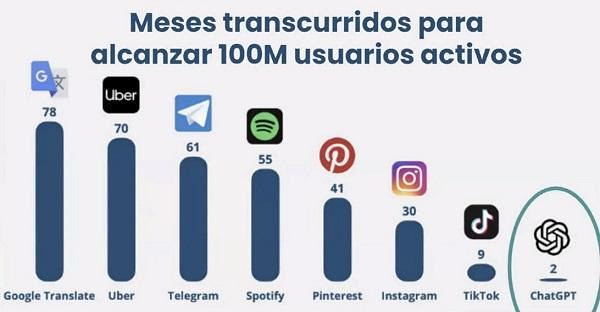
\includegraphics[width=0.4\textwidth]{./figuras/100millonesUsuariosChatgpt.jpeg}
            \source{\cite{PrimerosMesesChat2023}}
            \label{fig:crecimiento_chatgpt}
        \end{figure}

        \begin{figure}[h]
            \caption[Interfaz web de ChatGPT]{Interfaz web de ChatGPT}
            \centering
            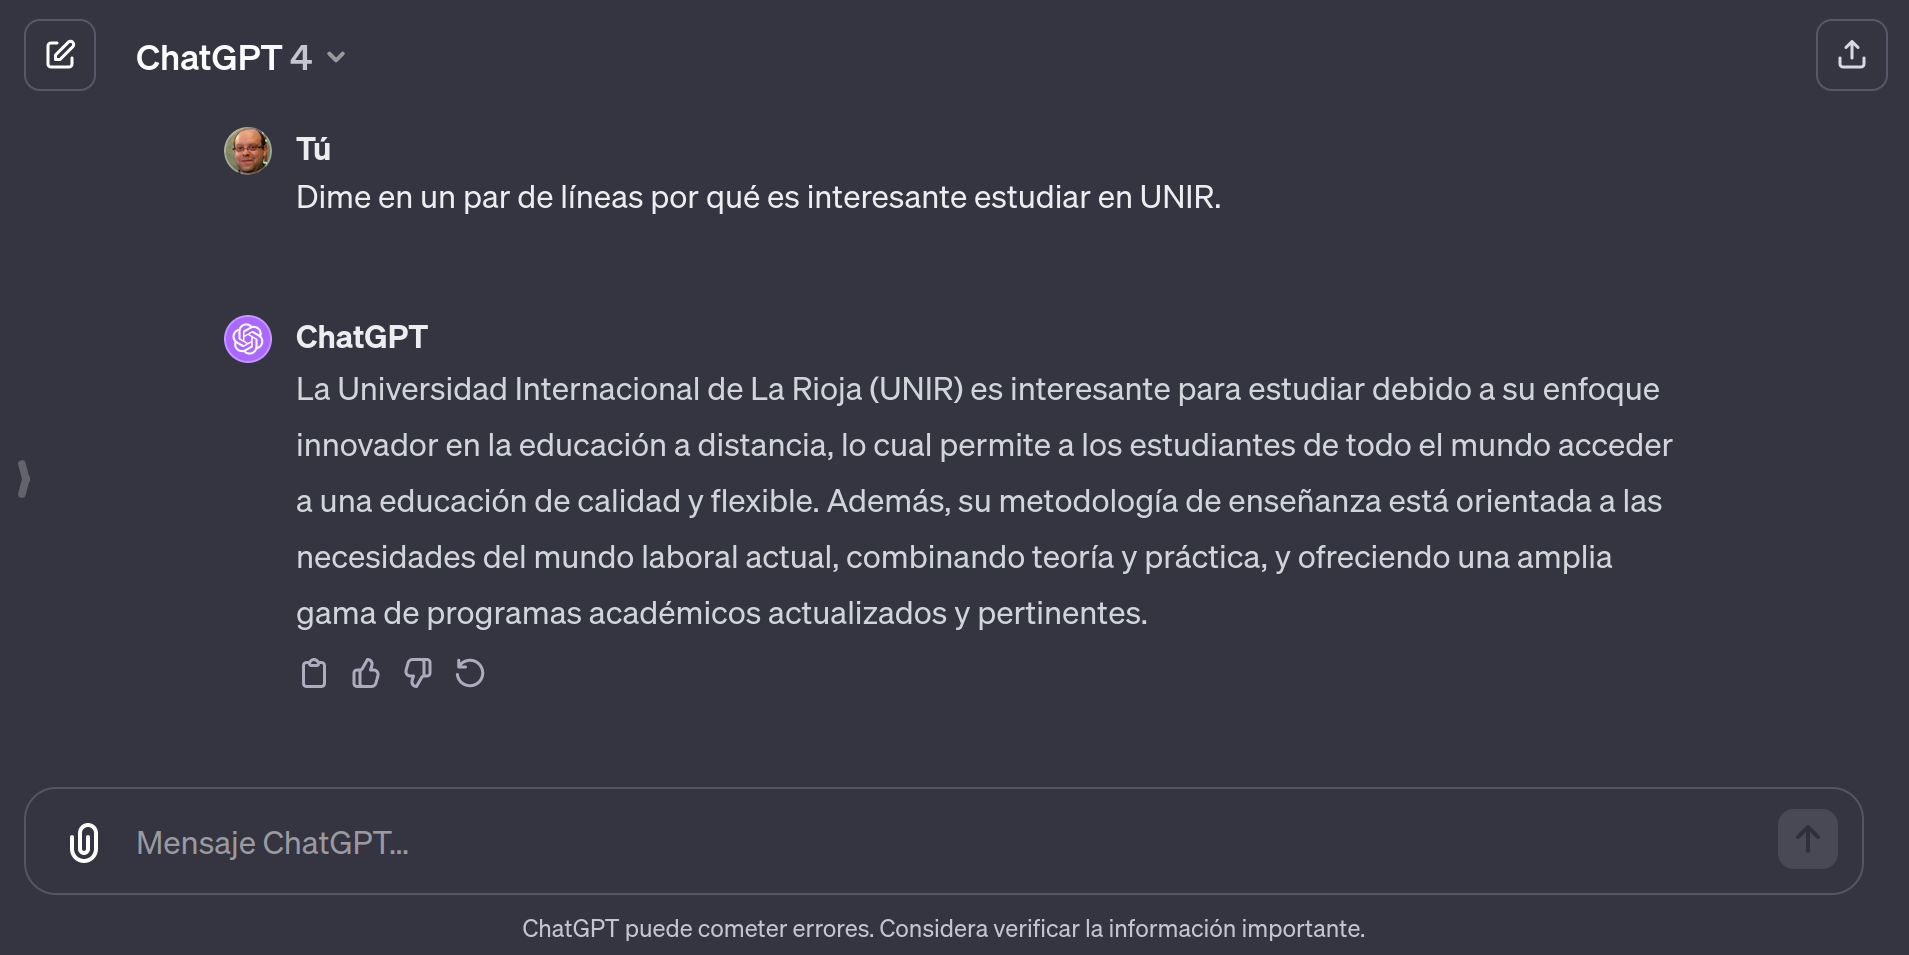
\includegraphics[width=0.4\textwidth]{./figuras/interfaz_chatgpt.png}
            \source{Imagen del autor}
            \label{fig:chatgpt}
        \end{figure}

        \paragraph{\textit{Playground.}} Esta herramienta permite interactuar con los modelos de lenguaje de OpenAI de forma más flexible que ChatGPT. En ella se pueden introducir \textit{prompts} de texto, así como seleccionar el modelo de lenguaje a utilizar, el número de respuestas a obtener, la \textit{temperatura} de generación, la presencia o ausencia de \textit{stopwords}, y la presencia o ausencia de \textit{top\_p sampling}, todos ellos parámetros avanzados en la interacción con los LLM (véase \ref{sec:hiperparametros_controlables}), sobre los que no existe ningún control por parte del usuario en la versión web de chatGPT. En la figura \ref{fig:playground} se puede observar la interfaz de Playground, donde el usuario puede introducir un \textit{prompt} de sistema, así como un mensaje de usuario, y obtener una respuesta del modelo de acuerdo a los parámetros seleccionados de \textit{temperatura} y \textit{top\_p sampling}. Esta herramienta es muy útil para la experimentación de esta y otras investigaciones con LLM, ya que permite una interacción más flexible con los LLM.

        \begin{figure}[h]
            \caption[Interfaz de \textit{Playground} de OpenAI]{Interfaz de \textit{Playground} de OpenAI}
            \centering
            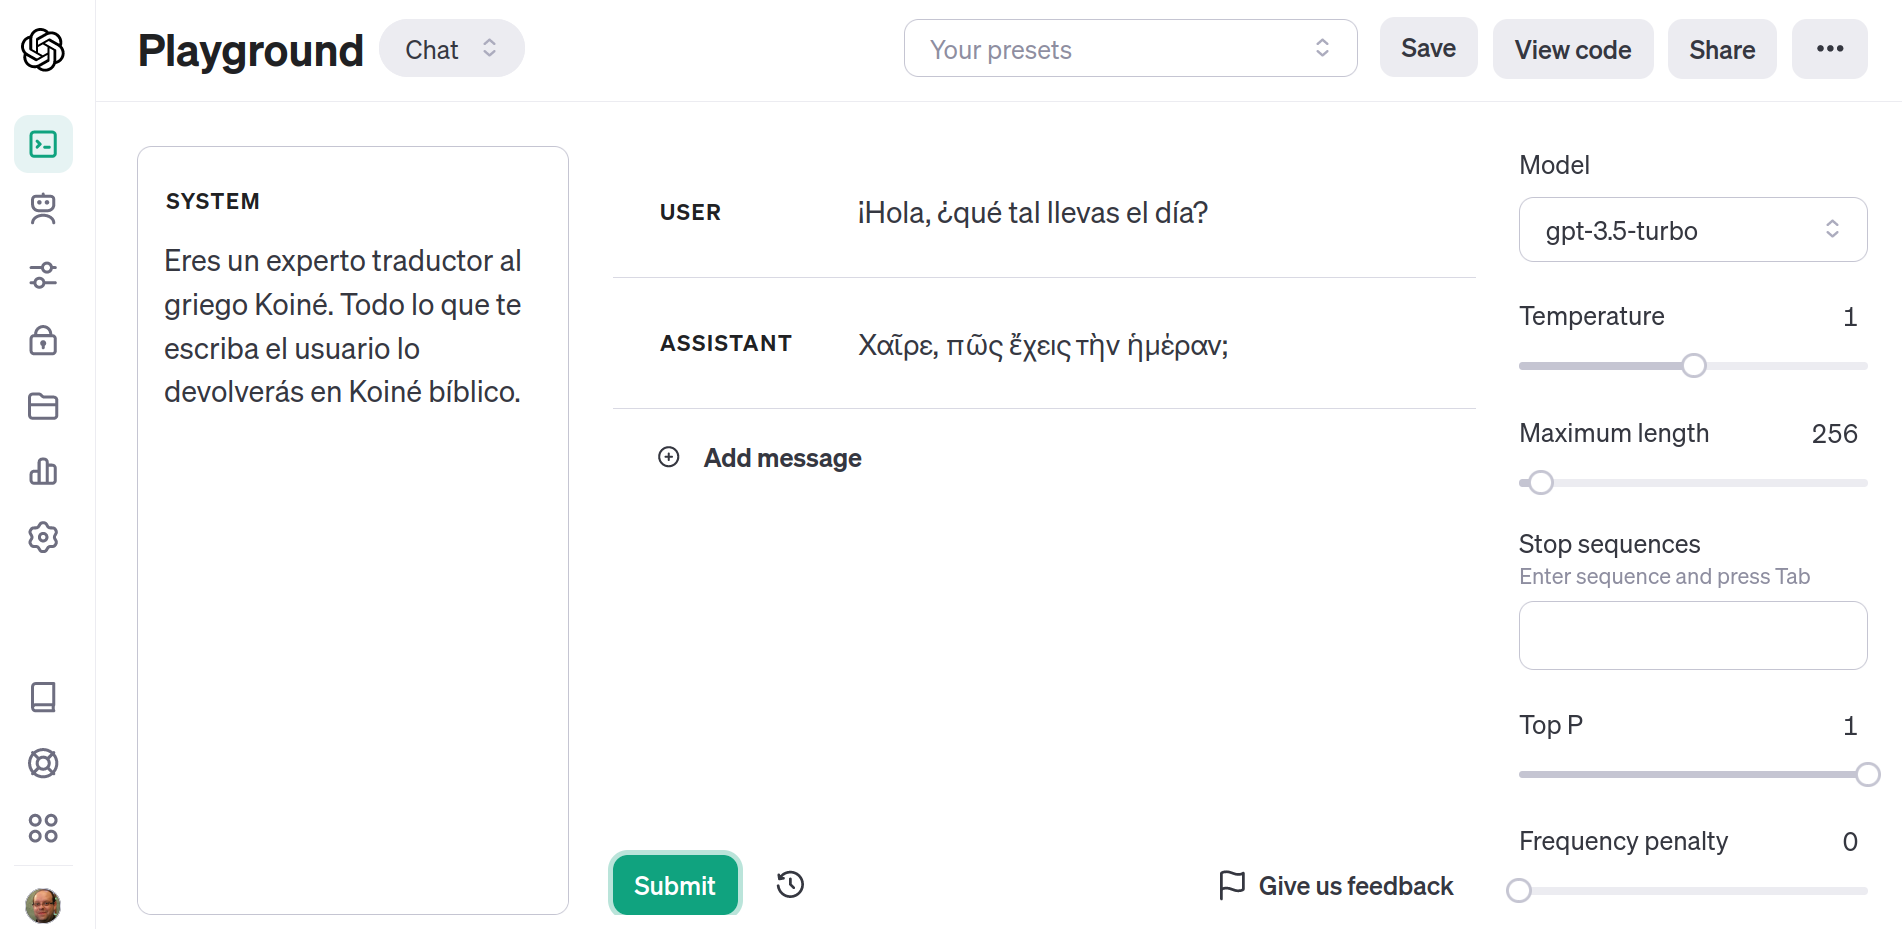
\includegraphics[width=0.4\textwidth]{./figuras/interfaz_playground.png}
            \source{Imagen del autor}
            \label{fig:playground}
        \end{figure}

        \paragraph{API de OpenAI.} La herramienta \textit{Playground} no es sino la antesala de la API de OpenAI. \textit{API}, del inglés \textit{Application Programming Interface}, es un conjunto de funciones y procedimientos que ofrece una biblioteca para ser utilizado por otro software como una capa de abstracción. En el caso de OpenAI, la API permite la interacción con los LLM de forma programática, es decir, mediante código. Esto permite una interacción absolutamente flexible a la par que potente con los LLM, ya que se pueden automatizar procesos, y se puede interactuar con los LLM de forma más rápida y eficiente. La API de OpenAI permite la interacción con diversos modelos de lenguaje basados en GPT-3 y GPT-4, así como con el modelo de generación de imágenes DALL-E 3. En la figura \ref{fig:api} se puede observar un ejemplo de interacción con la API de OpenAI, en el que se introduce un \textit{prompt} de sistema, otro de usuario, se ajustan los hiperparámetros y se obtiene una respuesta del modelo.

        \begin{figure}[h]
            \caption[Ejemplo con API de OpenAI]{Ejemplo con API de OpenAI}
            \centering
            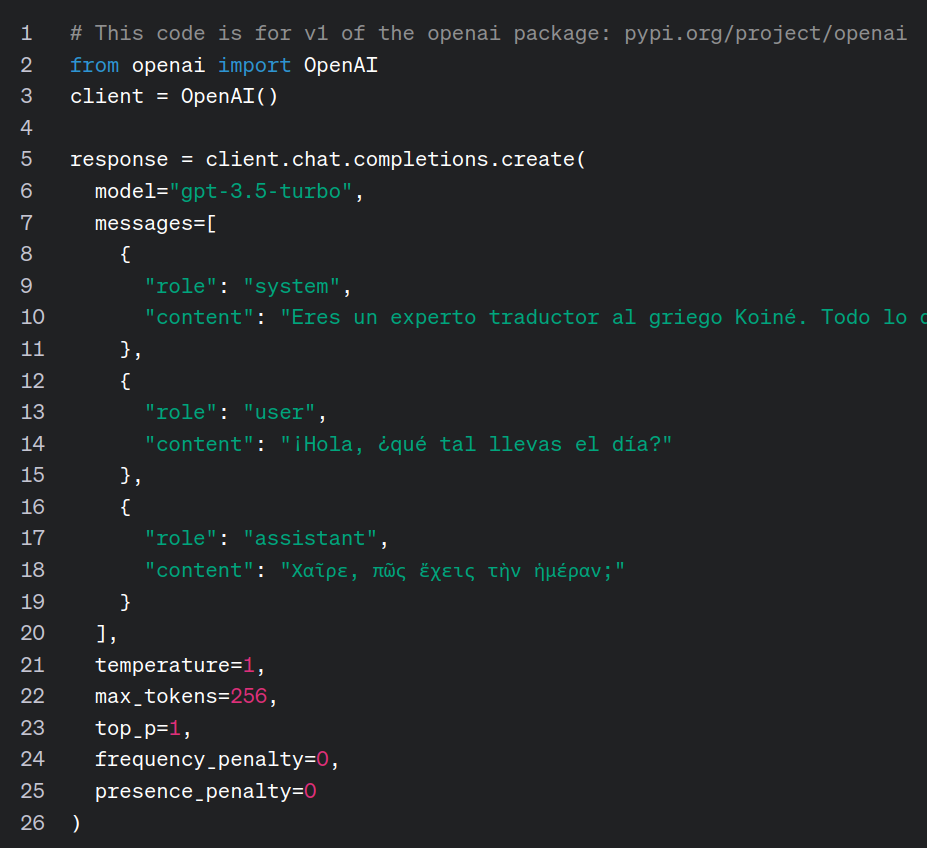
\includegraphics[width=0.4\textwidth]{./figuras/ejemplo_API.png}
            \source{Imagen del autor}
            \label{fig:api}
        \end{figure}

    \subsubsection{Python como lenguaje de programación}

Para llevar a cabo la experimentación en esta investigación, se utilizará el modelo GPT-4 proporcionado por OpenAI a través de su API. GPT-4 es, en el momento en que se escribe este texto, el modelo de lenguaje a gran escala más avanzado y potente disponible públicamente. Esta elección garantiza la interacción con una tecnología de vanguardia en el campo del procesamiento del lenguaje natural y el \textit{Deep Learning}. La API de OpenAI permite una interacción flexible y eficiente con el modelo, facilitando la introducción de \textit{prompts} y la recopilación de respuestas en tiempo real.

\subsection{Exploración de posibles interfaces de interacción humano-IA}
De algún modo, esta será la guia de la investigación. A partir de las posibilidades de interacción con los LLM, ofrecidas principalmente por la API de OpenAI, se explorarán las posibilidades de interacción con los LLM, y se diseñarán \textit{prompts} para interactuar con el modelo de cara a la composición musical por medio de código.

% Seguir revisando por aquí.

\subsection{Experimentación con \textit{prompts}}
Se realizarán múltiples sesiones de experimentación, en las cuales se introducirán diversos \textit{prompts} tanto de sistema como de usuario para interactuar con el LLM.

\subsection{Análisis cuantitativo}
Una vez recopilados los resultados, se llevará a cabo un análisis cuantitativo para determinar métricas como el porcentaje de respuestas correctas desde el punto de vista sintáctico y la calidad artística del output.

\subsection{Análisis cualitativo y reflexión}
Además del análisis cuantitativo, se reflexionará sobre las interacciones, las respuestas obtenidas y la experiencia durante el proceso, proporcionando hallazgos cualitativos sobre la interacción con los LLM.

\subsection{Comparación y reflexión final}
Se realizará una reflexión comparativa sobre la influencia de los LLM en el proceso creativo en contraste con creaciones realizadas sin su intervención. También se discutirán las implicaciones, limitaciones y posibles aplicaciones futuras de los descubrimientos de la investigación.